% Figure 5 — WRI vs. Attack Strength for five attack types (with 95% CI)

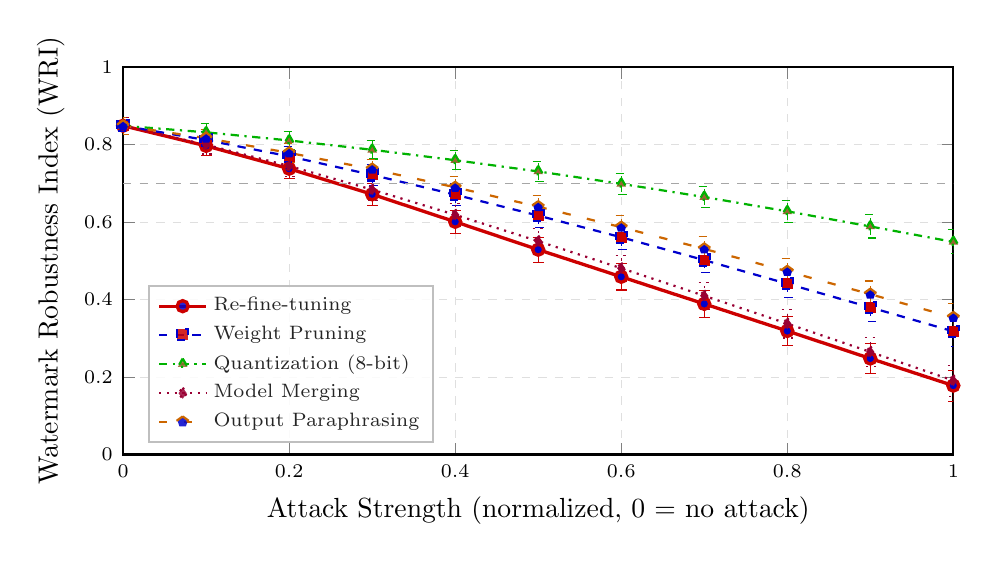
\begin{tikzpicture}
\begin{axis}[
  width=\columnwidth,
  height=6.5cm,
  xlabel={Attack Strength (normalized, 0 = no attack)},
  ylabel={Watermark Robustness Index (WRI)},
  ymin=0.0, ymax=1.0,
  xmin=0.0, xmax=1.0,
  xtick={0,0.2,0.4,0.6,0.8,1.0},
  xticklabel style={font=\scriptsize},
  yticklabel style={font=\scriptsize},
  legend pos=south west,
  legend style={font=\scriptsize, cells={anchor=west},
    fill=white, fill opacity=0.85, draw=gray!50},
  grid=major,
  grid style={gray!25, dashed},
  thick,
  mark size=2.0pt,
]

% Re-fine-tuning
\addplot+[
  color=red!80!black, mark=*, solid, very thick,
  error bars/.cd, y dir=both, y explicit
] coordinates {
  (0.0,0.849)+-(0,0.022)
  (0.1,0.797)+-(0,0.024)
  (0.2,0.738)+-(0,0.026)
  (0.3,0.672)+-(0,0.028)
  (0.4,0.601)+-(0,0.030)
  (0.5,0.529)+-(0,0.032)
  (0.6,0.459)+-(0,0.034)
  (0.7,0.389)+-(0,0.035)
  (0.8,0.319)+-(0,0.037)
  (0.9,0.248)+-(0,0.038)
  (1.0,0.178)+-(0,0.040)
};
\addlegendentry{Re-fine-tuning}

% Weight Pruning
\addplot+[
  color=blue!80!black, mark=square*, dashed, thick,
  error bars/.cd, y dir=both, y explicit
] coordinates {
  (0.0,0.849)+-(0,0.022)
  (0.1,0.812)+-(0,0.023)
  (0.2,0.770)+-(0,0.025)
  (0.3,0.722)+-(0,0.027)
  (0.4,0.671)+-(0,0.028)
  (0.5,0.617)+-(0,0.030)
  (0.6,0.561)+-(0,0.032)
  (0.7,0.502)+-(0,0.033)
  (0.8,0.441)+-(0,0.035)
  (0.9,0.380)+-(0,0.036)
  (1.0,0.318)+-(0,0.038)
};
\addlegendentry{Weight Pruning}

% Quantization (8-bit)
\addplot+[
  color=green!70!black, mark=triangle*, dash dot, thick,
  error bars/.cd, y dir=both, y explicit
] coordinates {
  (0.0,0.849)+-(0,0.022)
  (0.1,0.832)+-(0,0.022)
  (0.2,0.811)+-(0,0.023)
  (0.3,0.787)+-(0,0.024)
  (0.4,0.760)+-(0,0.025)
  (0.5,0.731)+-(0,0.026)
  (0.6,0.699)+-(0,0.027)
  (0.7,0.665)+-(0,0.028)
  (0.8,0.628)+-(0,0.029)
  (0.9,0.589)+-(0,0.030)
  (1.0,0.549)+-(0,0.031)
};
\addlegendentry{Quantization (8-bit)}

% Model Merging
\addplot+[
  color=purple!80!black, mark=diamond*, dotted, thick,
  error bars/.cd, y dir=both, y explicit
] coordinates {
  (0.0,0.849)+-(0,0.022)
  (0.1,0.800)+-(0,0.024)
  (0.2,0.745)+-(0,0.026)
  (0.3,0.684)+-(0,0.028)
  (0.4,0.619)+-(0,0.030)
  (0.5,0.551)+-(0,0.032)
  (0.6,0.481)+-(0,0.034)
  (0.7,0.410)+-(0,0.035)
  (0.8,0.338)+-(0,0.037)
  (0.9,0.265)+-(0,0.038)
  (1.0,0.191)+-(0,0.040)
};
\addlegendentry{Model Merging}

% Output Paraphrasing
\addplot+[
  color=orange!80!black, mark=pentagon*, loosely dashed, thick,
  error bars/.cd, y dir=both, y explicit
] coordinates {
  (0.0,0.849)+-(0,0.022)
  (0.1,0.817)+-(0,0.023)
  (0.2,0.779)+-(0,0.024)
  (0.3,0.737)+-(0,0.025)
  (0.4,0.690)+-(0,0.027)
  (0.5,0.640)+-(0,0.028)
  (0.6,0.587)+-(0,0.030)
  (0.7,0.531)+-(0,0.031)
  (0.8,0.473)+-(0,0.033)
  (0.9,0.414)+-(0,0.034)
  (1.0,0.354)+-(0,0.036)
};
\addlegendentry{Output Paraphrasing}

% Threshold line
\draw[gray!70, dashed, thin] (axis cs:0,0.70) -- (axis cs:1.0,0.70)
  node[right, font=\scriptsize, gray]{$\tau_{\mathrm{WRI}}=0.70$};

\end{axis}
\end{tikzpicture}
